\section{Computer Intelligence Solution}
	The software system consists basically of five modules: AI, LogPlayer, Simulated World,
Support Simulation and Transmission. The modules were implemented using the Microsoft Visual
Studio 2010 IDE, that allows a single solution integrated of projects in different programming
languages (e.g. CSharp, C++), making the project more flexible for other programmers giving
continuity to the implementation.

	We chose to adopt the fragmentation of the software project into modules to facilitating
the implementation team. A UDP socket interface was adopted for communication between most modules
giving independence to them. Some interfaces like between AI Module and Support Simulation Module,
that need high performance, don't communicate using the UDP Socket interface. Figure \ref{fluxogramaSoftware}
shows the block diagram of the software system.

\begin{figure}[thpb]
     \centering
%TODO update image  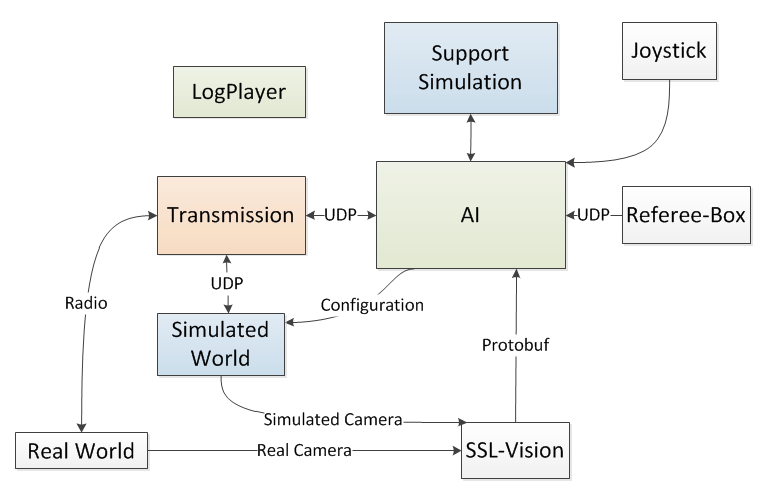
\includegraphics[scale=0.55]{img/fluxogramaSoftware.png}
     \caption{Block diagram of the software system}
     \label{fluxogramaSoftware}
\end{figure}

\subsection{Artificial Intelligence}
	This is the largest and most complex software module. It is responsible for the following features:
\begin{itemize}
\item Collect, interpret and filter data from the Referee-Box, SSL-Vision, Transmission Module (real world or simulated), Support Simulation Module and Joystick;
\item Take high level decisions to define the actions that robot should do (i.e., to find the position
and orientation that robot has to reached, find the force to kick the ball, find the torque to dribble the ball);
\item Use the Support Simulation Module to create a planning;
\item Make a short future preview of the world (real or simulated) using data from the sensors (encoder, camera, infra-red);
\item Make the configuration of the simulation environment Simulated World (setting bodies existing in the simulation);
\item Control position and orientation of the robot defining which speeds the robot actuators (motor,
kicker and dribbler) must reach. These speeds will be passed to Transmission Module to be sent to the World (simulated or real);
\end{itemize}

	Among the many reactive behavioural control architectures, we have chosen STP (Skills, Tactics and Plays)
architecture \cite{STP}. In order to create a plan, we use two algorithms: Minimax \cite{minimax} and
BK-BGT (Behavioural Kinodynamic Balanced Growth Trees) \cite{zickler}. These algorithms works as Play on the
STP architecture.

	On the implementation of Minimax, the players agents are based on objective (assessed by an objective function)
and the minimax algorithm is used to define which heuristics (Skills, Tactics and Plays) to use. The objective function
consider several factors: distance from the ball to the opposing goal, distance from the ball to the goal together,
distance from the ball to the opposing players, among others. The two algorithms use the Support Simulation Module to
creating a Physics-Based Robot Motion Planning.

Extended Kalman Filter (EKF) \cite{ekf} is used to offset the effects induced by time
latency in that accumulates in vision systems, AI, communication and execution of commands for the robot.

%XMLCONFIG, CONTROL POSE, The Communication provides an interface with a joystick to both the real robot when the simulation can be ccontrolled by one person.

\subsection{LogPlayer Module}
	This module is important to debug the planning algorithms. AI Module creates
a log file with all the information necessary to describe the tree planning, so using
the LogPlayer Module we can play the log files to visualize all possible solutions
present in the tree planning.

\begin{figure}[thpb]
	\centering
	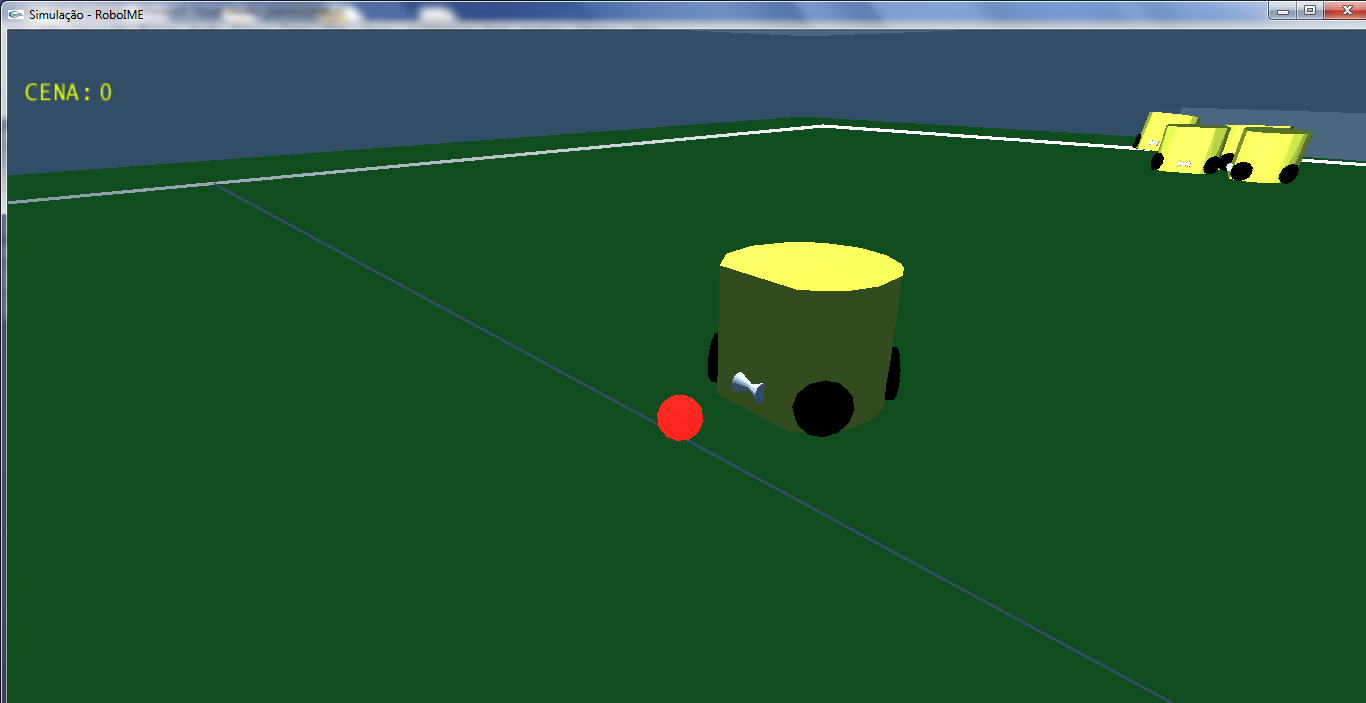
\includegraphics[scale = 0.36]{img/roboSim1.png}
	\caption{Simulated robot.}
	\label{roboSim}
\end{figure}

\subsection{Support Simulation Module}

	This module is part of F180 environment simulator. It simulates the physics of bodies presented in a match from the Small Size Robot League. Its also possible to make the control of robot actuators (motor, kicker and dribbler).

	The simulator was developed using the PhysX Engine, that enables high performance processing physics calculations in a GPU. Figure \ref{roboSim} shows the robot in the simulator. This module can provide long-terms predictions, in opposition to the Kalman Filter that provides a short-term prediction.

\subsection{Simulated World Module}
	This module is also part of the simulator designed to F180's environment. But this module replaces the
Real World, when it is not convenient to use it. Thus this module receives through UDP sockets the speeds that
the actuators of the robot must reach, the simulator has an internal controller to calculate the torque required
to be applied to the actuators to achieve the desired speed (like real robot).

\begin{figure}[thpb]
	\centering
%	\includegraphics[scale = 0.36]{simulacao1.png}
	\caption{Simulation environment of the F180.}
	\label{prototype}
\end{figure}

	The AI Module can configure the simulation environment of the Simulated World Module just sending an XML file,
via UDP Socket, containing information for the construction of bodies in the simulator. This module has two simulated
cameras which provide input to SSL-Vision, we use two OpenGL cameras and the images are sent through TCP sockets.

\subsection{Transmission Module}
	This module is responsible for delivering the speed to actuators and receiving status of the robot, such as real velocity
of each motor, kick sensor status and power supply status, via radio in Real World or via UDP socket in Simulation World. This
module is coded in CSharp language using the interface development Microsoft Visual Studio 2010 IDE.

\subsection{Path Planning}

Path planning algorithm is based on the theory of Artificial Potential Field \cite{CPA}, which has as its fundamental principle driving
the robot in an artificial force field generated by obstacles and the target. The potential (gradient) should be continuous.
The obstacles (other robots) and the target (certain objective local) generating fields of repulsion and attraction, respectively,
obtaining a movement by which avoids obstacles and possibly reach your goal.

%FAZER A PARTE DO A-ESTRELA
